		The set of four traditional playing card suits are split into two further subcategories; diamonds and hearts in red, and clubs and spades in black. This information can be determined beforehand when classifying a card and used to reduce the suit symbol search space, as well as help increase detection accuracy. For example, when compared side by side, the hearts and spades suits both appear similar due to their curves and large surface area, with the spaces symbol appearing similar to a heart when viewed upside down.

		\begin{figure}[H]
			\centering
			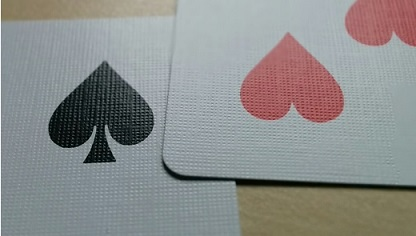
\includegraphics[width=0.6\linewidth]{chris/image16}
			\caption{Hearts and Spades can look similar, highlighting the usefulness of colour information integration.}
			\label{fig:colours}
		\end{figure}

		% TODO: Also to divide HoM search space by 2
		Using this line of thinking, the top left and bottom right corners of the card are evaluated according to their `redness'. A card that has a large surface area of `redness' is likely to be either a diamonds card or a hearts card. The first stage in this step of classification is to make the background of the card completely black. The reason behind this is that a white pixel is as bright as it is due to a large red component, along with large green and blue components also. By transforming all white pixels above a threshold into black pixels, only the majority-red pixels will remain. This is implemented as shown below:
		
		\begin{lstlisting}

//For all pixels...
for(int y = 0; y < input_size.height; y++)
{
	for(int x = 0; x < input_size.width; x++)
	{
		//Get BGR values
		int b = in_data[(y)*input.step + (x)*input_channels + 0];
		int g = in_data[(y)*input.step + (x)*input_channels + 1];
		int r = in_data[(y)*input.step + (x)*input_channels + 2];

		//Set output pixel
		if(b > white_level && g > white_level && r > white_level)
		{
			//Make it black
			out_data[(y)*output.step + (x)*output_channels + 0] = 0;
			out_data[(y)*output.step + (x)*output_channels + 1] = 0;
			out_data[(y)*output.step + (x)*output_channels + 2] = 0;
		}
		else
		{
			//Leave pixel as it is
		}
	}
}
		\end{lstlisting}

		The result of this operation is illustrated below in Figure~\ref{fig:whitebg}:
		\begin{figure}[H]
			\centering
			\begin{subfigure}[b]{0.4\textwidth}
				\centering
				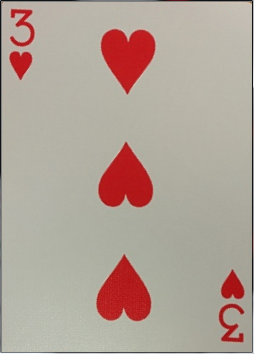
\includegraphics[width=\textwidth]{chris/image17}
				\caption{}
			\end{subfigure}
			\begin{subfigure}[b]{0.4\textwidth}
				\centering
				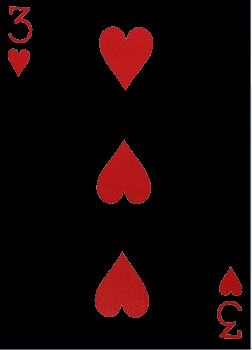
\includegraphics[width=\textwidth]{chris/image18}
				\caption{}
			\end{subfigure}
			\caption{An isolated card (a) with white background pixels removed (b).}
			\label{fig:whitebg}
		\end{figure}

		Once this is complete, the image is then filtered to remove all green and blue component values, leaving a purely red image:
		
		\begin{lstlisting}

//For all pixels...
for(int y = 0; y < input_size.height; y++)
{
	for(int x = 0; x < input_size.width; x++)
	{
		//Set output pixel              
		out_data[(y)*output.step + (x)*output_channels + 0] = new_value;    //B
		out_data[(y)*output.step + (x)*output_channels + 1] = new_value;    //G 
	}
}
		\end{lstlisting}

		where \code{new_value} is set to 0 (black). The red component is left untouched. The result is shown below:

		\begin{figure}[H]
			\centering
			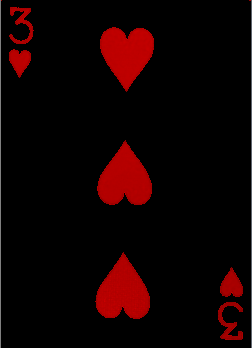
\includegraphics[width=0.4\textwidth]{chris/image19}
			\caption{An isolated card (a) with white background pixels removed (b).}
			\label{fig:redchan}
		\end{figure}

		The final step in this suit colour processing stage is to evaluate whether the top-left and bottom-right corners are sufficiently high in red surface area that they can be classified as belonging to a red suit. This final step of implementation is shown below (abbreviated):

		\begin{lstlisting}

bool is_red_suit_by_corners(cv::Mat input, int base_threshold, int target_regions, float perc_red)
{
	...

	//Get four corner regions
	int region_width = Card::TOP_CORNER_RECT.width;
	int region_height = Card::TOP_CORNER_RECT.height;

	//Create region matrices, top left, bottom right...
	cv::Mat regions[2] = {
		input(Card::TOP_CORNER_RECT),
		input(Card::BOTTOM_CORNER_RECT)
	};

	//For all regions...
	for(int i = 0; i < 2; i++)
	{
		//Reset totals
		red = 0; green = 0; blue = 0;

		//Pointer to data
		uchar *data = (uchar*)regions[i].data;

		//Get region channels once for speed
		int region_channels = regions[i].channels();

		//For all pixels...
		for(int y = 0; y < region_height; y++)
		{
			for(int x = 0; x < region_width; x++)
			{
				//Get values
				int b = data[(y)*regions[i].step + (x)*region_channels + 0];
				int g = data[(y)*regions[i].step + (x)*region_channels + 1];
				int r = data[(y)*regions[i].step + (x)*region_channels + 2];

				if(max(r, g, b) == r && r > base_threshold)
				{
					red++;
				}
				else if(max(r, g, b) == g && g > base_threshold)
				{
					green++;
				}
				else if(max(r, g, b) == b && b > base_threshold)
				{
					blue++;
				}
				else {
					//No action
				}
			}
		}

		//Compute result
		float total = (float)region_width * (float) region_height;
		float match_perc = (float) red / total;
		regions_red[i] = (red > blue && red > green) && match_perc > perc_red;
		
		...
	}

	//Count number of red regions
	int count = 0;
	for(int c = 0; c < 2; c++)
	{
		if(regions_red[c] == true)
		{
			count++;
		}
	}

	...

	return count >= target_regions;
}
		\end{lstlisting}

		Thus if both the examined regions are found to be majority red above the parametrised percentage specified, the function returns \code{true}, meaning the card suit is a red suit, either diamonds or hearts. The result structure is then assigned the appropriate colour enumeration constant.

		When called as part of card isolation, the call appears as below:

		\begin{lstlisting}

card->detected_colour = is_red_suit_by_corners(working, 100, 2, 0.10F) ? Card::RED : Card::BLACK;
		\end{lstlisting}